\chapter{巨洞}
\label{cha:void}

\section{引言}
广义上的巨洞是宇宙中密度较低且不存在大质量暗物质晕或高光度星系的较大区域。因为观测极限星等或宇宙学数值模拟的质量分辨率的限制,巨洞的内部可能会存在小质量暗物质晕或低光度星系,并不是完全空无一物~\cite{Patiri2006372}。在巡天观测或宇宙学数值模拟中,巨洞并不像暗物质晕或星系一样有相对背景环境非常明显区别,所以巨洞不像暗物质晕或星系一样可以被非常直观的被观测。因此不同人研究巨洞时会从自己感兴趣的研究及手头可以使用的数据出发去定义巨洞并开发相应的工具去寻找巨洞,目前学界并不存在对巨洞的统一定义。因为巡天观测中可以非常直观的确定星系的位置,所以一些工作基于星系在空间中的离散分布来定义巨洞。使用宇宙学数值伪星表可以直接计算密度场的分布,另一些工作认为应该直接从密度场出发去寻找真正的低密度的区域来定义巨洞,这些类巨洞的定义更直接。但是目前的星系红移巡天观测中只能得到星系的位置,需要间接的利用星系的分布来估计宇宙的密度场,而弱引力透镜的观测虽然可以得到一些区域的密度场,但是其精度很低。因此基于密度场去定义巨洞的研究很难适用于真实观测的数据,只能使用宇宙学数值模拟进行一些理论研究。本章总结了不同的工作中定义巨洞的方法相和相应的一些研究。

%What one can observe is the galaxies. So most of the study define voids based on the distribution of galaxies. It is possible to measure the density field in a simulation, so some works define voids as the real under density region with the simulated density field. One may expect to measure the density field of the Universe from weak lensing survey, but so far the resolution of the weak lensing result is not good enough. There are different kinds of void finders for different research topics with cosmic void. Our group developed a novel parameter-free cosmological void finder, which is very computationally efficient \citep[][]{Zhao2016DIVE}.
%\section{Void BAO}
\section{巨洞的发现及早期研究}
第一个被观测到的巨洞The Giant Bo\"otes voids

CfA红移巡天中发现的巨洞

\section{The Void Finder developed by \cite{El-Ad1997}}

%\citealt{El-Ad1997} believed that the main fetures of the cosmological large scale structures are voids surrounded by walls. Walls are generally 2D thin structures with high density constructed by galaxies, and the boundary of the ellipsoidal voids. Galaxies in the walls are named "wall galaxies" while the no-wall galaxies are labeled "field galaxies". The voids are only empty of wall galaxies but there might be field galaxies inside. And the galaxies inside voids are void galaxies which are subsamples of field galaxies.

%The first step of the void finder is to identify the wall galaxies and field galaxies, which is done by the WALL BUILDER. Then the voids are located by the VOID FINDER in the distribution of wall galaxies. There are three parameters in this method: $n$ and $\beta$ are used to determine the field galaxies and $\xi$ is for searching voids.

\section{用巨洞的数密度限制$\sigma_8$和$h\, \Omega_m$}

巨洞可以被定义为在三维空间离散分布的样本(暗物质晕或星系)中许多半径最大且不互相重叠的空心球~\cite{Patiri2006HB,BPP09}。基于这个定义,使用HB void finder~\cite{Patiri2006HB} 可以从离散分布的星系星表中获得巨洞概率函数(Void Probability Function,VPF)和巨洞样本。而巨洞累积数密度(accumulative void number density)可以用来限制宇宙学参数$\sigma_8$和$h\, \Omega_m$~\cite{BPP09}。

\subsection{HB void finder}
\label{sec:hb}

这一节介绍HB void finder如果从离散分布的样本中寻找巨洞:
\begin{description}
%\item[1.]filter the galaxy mocks with the veto flag and fiber collision flag.
\item[1.] 选择巨洞的最小半径$R_{\rm min}$,将N个半径为$R_{\rm min}$的球随即放在样本空间内。检查这N个球是否空心,其中$N_e$个是空心球。巨洞的VPF($R_{\rm min}$) = $N_e$/N。
\item[2.] 空间中四个点可以唯一的确定一个球的球心和半径。寻找距离每个空心球球心最近的四个样本,计算四个样本所唯一确定的球的中心位置和半径,得到$N_e$个新的球,这些新的球并不一定是空心的。检查这些球是否空心,其中$N_{2}$个是空心的。
\item[3.] 从$N_{2}$个新的空心球中选择不互相重叠的最大的球,这些最大的不互相重叠的空心球就是HB void finder的最终结果。
\end{description}

\begin{figure}
\centering
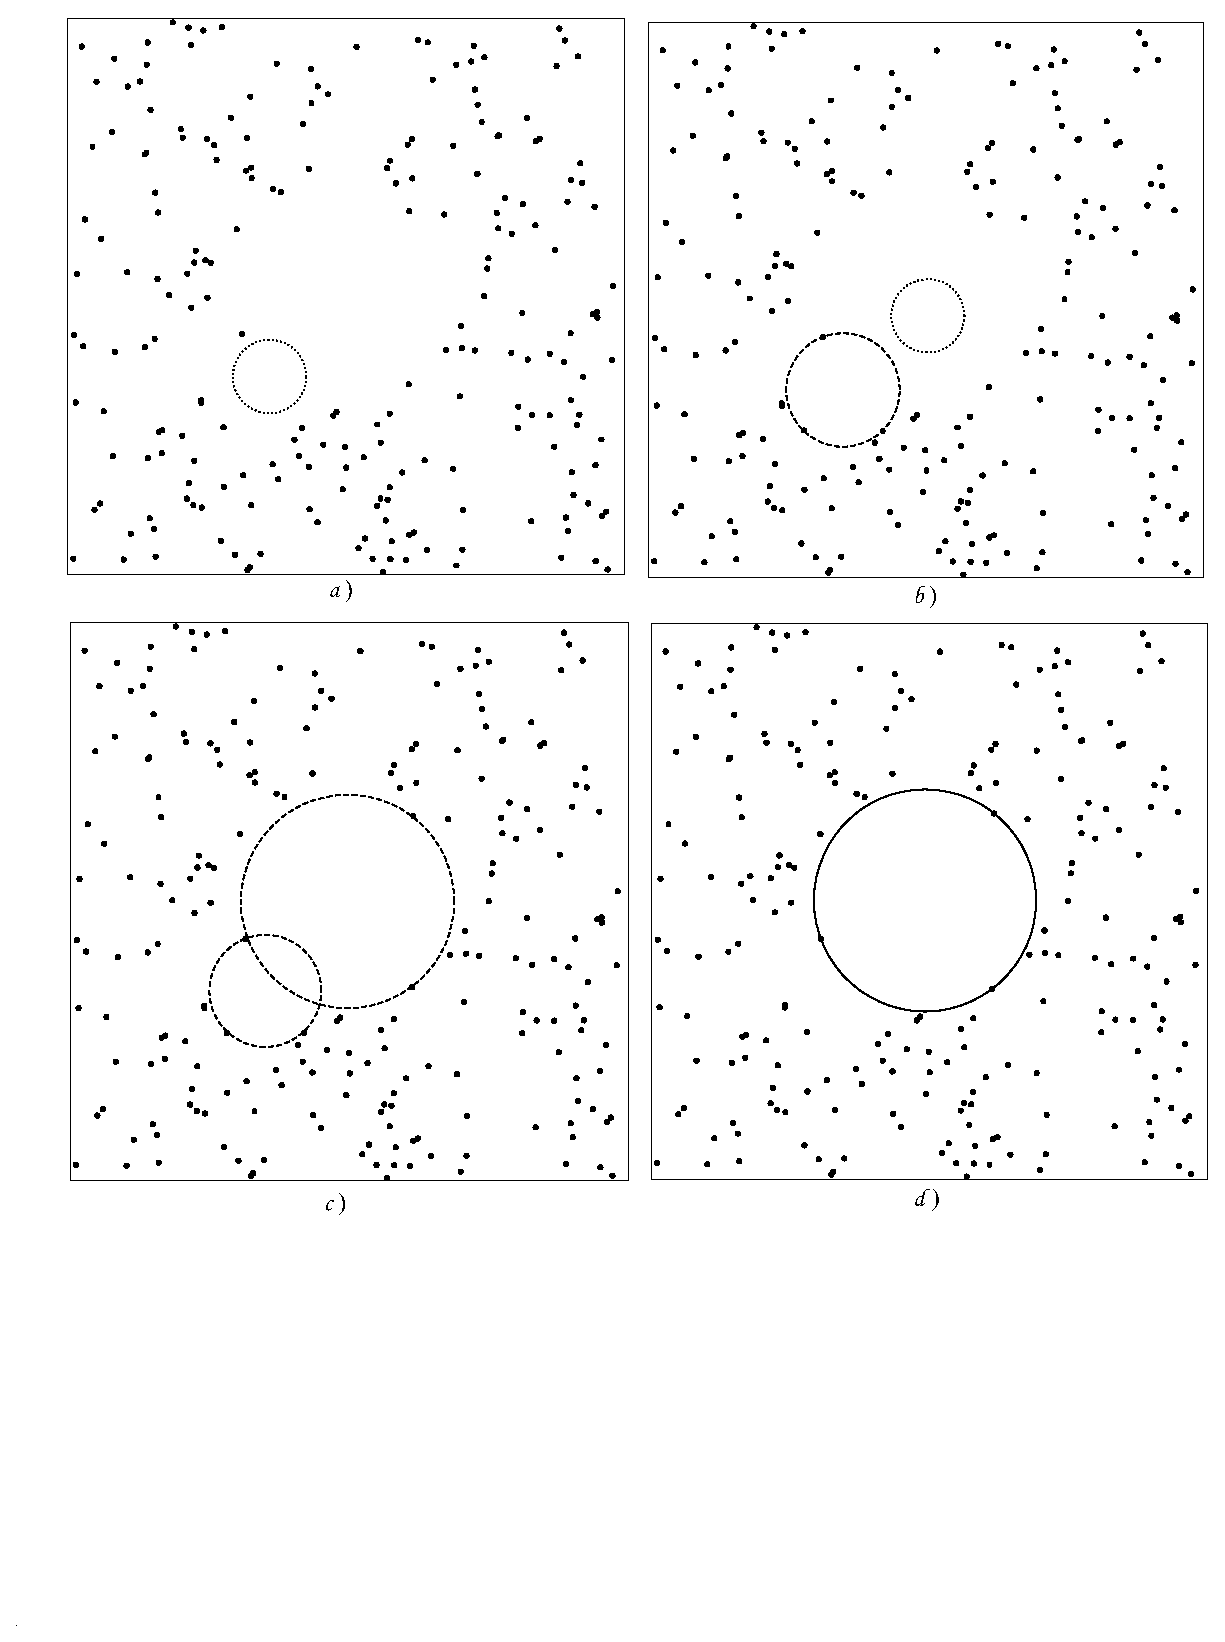
\includegraphics[width=.9\textwidth]{hb.eps}
\caption{HB Void Finder的工作流程:$a)$ 将半径为$R_{\rm min}$的球随即放在样本空间内;
$b)$ 如果随即放置的球为空心,则寻找距离球心最近的四个样本并计算新的中心和半径,并检查其他随机放置的球是否空心;$c)$ 对所有随机放置的空心球重复上一步,最终得到所有新的空心球;$d)$ 新的空心球中如果两个球互相重叠,则将较小的移除,直到只留下不互相重叠的最大的空心球。(文献 ~\inlinecite{Patiri2006HB} 中Figure A2)}
\label{fig:hb}
\end{figure}

\subsection{用巨洞的数密度限制$\sigma_8$和$h\, \Omega_m$的理论模型}


\section{Explicit computation of $P_{\lowercase{n}}(\lowercase{r})$}

%\appendix{Appendix A}\\
%\renewcommand{\theequation}{A-\arabic{equation}}
In this section we show the detailed procedure for computing $P_n(r)$ and the void statistics for given values of $\sigma_8$ and $\Gamma$.

\begin{equation}
P_n(r) = \frac{1}{n!} \int_{-7}^{0} P(\delta_l,r) [u(\delta_l)]^n e^{[-u(\delta_l)]} d\delta_l   \label{eq:eqA1}
\end{equation}

\begin{equation}
u(\delta_l) = \bar{n} V [1+{\rm DELF}(\delta_l,r)] A e^{-b\delta_l^2}    \label{eq:eqA2}
\end{equation}
${\rm DELF}$ is a function of $\delta_l$ and $r$ that gives the mean actual density contrast within a sphere with radius $r$ with enclosed 
linear density contrast $\delta_l$.

\begin{eqnarray}
{\rm DELF}(\delta_l,r) \equiv & \nonumber\\
 \frac{1+{\rm DELT}(\delta_l)}{| 1 - \frac{4}{21}[1+{\rm DELT}(\delta_l)]^{2/3}[\sigma(r[1+{\rm DELT}(\delta_l)]^{1/3})]^{2} |} &    \label{eq:eqA3}
\end{eqnarray}
where ${\rm DELT}(\delta_l)$ denotes the relationship between the actual and linear enclosed density contrasts in the spherical colapse model 
(see PBP06 for details).

\begin{equation}
1+{\rm DELT}(\delta_l) \simeq (1-0.607\delta_l)^{-1.66}   \label{eq:eqA4}
\end{equation}
$\sigma(Q)$ is the rms of the linear density contrast on a sphere with Lagrangian radius $Q$. In this equation, $\sigma(Q)$ is evaluated 
at $Q$ equal to $r[1+{\rm DELT}(\delta_l)]^{1/3}$. Explicit equations for $\sigma$ are given at the end of this Appendix.
$A$, $b$ in eq. (A2) are also functions of $\delta_l$ given by:

\begin{eqnarray}
 A \equiv &A(m,Q=r[1+{\rm DELT}(\delta_l)]^{1/3})  \times  \\
 &\times \left(\frac{D(z)\sigma_8}{0.9}\right)^{0.88} \left(\frac{\Gamma}{0.21}\right)^{0.343} \nonumber \\
 \nonumber\\
 b \equiv &b(m,Q=r[1+{\rm DELT}(\delta_l)]^{1/3})  \times   \\
 & \times \left(\frac{D(z)\sigma_8}{0.9}\right)^{-2.55} \left(\frac{\Gamma}{0.21}\right)^{-0.82} \nonumber \label{eq:eqA5}
\end{eqnarray} 
\\
where $A(m,Q)$, $b(m,Q)$ are functions of the mass of the objects and the Lagrangian radius of the regions being considered (that 
corresponding to an Eulerian sphere with radius $r$, see Rubi\~no et al. 2008):

\begin{eqnarray}
A(m,Q) = &[1.577 - 0.298 (\frac{Q}{8})] - \\
- &[0.0557 + 0.0447 (\frac{Q}{8})] {\rm ln}(m) -\nonumber\\
- &[0.00565 + 0.0018(\frac{Q}{8}][{\rm ln}(m)]^2\nonumber\\
\nonumber\\
b(m,Q) = &[0.0025 - 0.00146 (\frac{Q}{8})] + \\
+ &[0.121 - 0.0156(\frac{Q}{8})] \times \nonumber \\
\times & m^{[0.335 + 0.019 (\frac{Q}{8})]} \nonumber\\
\nonumber\\
m \equiv &\frac{M}{3.51 \times 10^{11} h^{-1}M_{\odot}}\left(\frac{0.21}{\Gamma}\right)    \label{eq:eqA6}
\end{eqnarray}
where $M$ is the mass of the objects, $D(z)$ in equations A5,A6 is the linear growth factor normalized to be 1 at present. The exponents determining the dependence on $A$, $b$ on $\sigma_8$ and redshift are slightly different from those given by Rubi\~no et al. (2008) but are within the precision afforded by the procedure used in that work. The exponents given here have been accurately fitted using numerical simulations. 

For dark matter halos, the values of $m$ entering in these last equations is defined by:
\begin{equation}
\bar{n}(>m)=\bar{n}_{sample}
\end{equation}
while for galaxies we have to use $m_g$ given in equation (\ref{eq:eq14}). The definition of $m$ and $m_g$ imply that these 
quantities have to be scaled with $\sigma_{8}$, $\Gamma$ and redshift. However, $m$ changes very little with these variables up to $z\sim 1$, so we 
chose to held it fixed. In the case of $m_g$ the scaling can be approximated by:

\begin{equation}
m_{g}(\sigma_{8},\Gamma,z) = m (1.124)^{(D(z)\sigma_{8}/0.9)(\Gamma/0.21)^{0.271})}
\end{equation}
 

We use for the probability distribution $P(\delta_l,r)$ of the linear density contrast within an Eulerian space given by Betancort-Rijo \& L\'opez-Corredoira (2002):

\begin{eqnarray}
P(\delta_l,r) = &\frac{exp\left[\frac{-1}{2} \frac{\delta_l^2}{(\sigma(r[1+{\rm DELF}(\delta_l,r)]^{1/3})^2}\right]}{\sqrt{2\pi}} \times \nonumber\\ 
\times &[1 + {\rm DELF}(\delta_l,r)]^{-(1-\frac{\alpha}{2})} \times \nonumber\\
\times &\frac{d}{d\delta_l} \left( \frac{\delta_l}{\sigma(r[1+{\rm DELF}(\delta_l,r)]^{1/3})}\right)\nonumber\\
\alpha(\delta_l,r) = &0.54 + 0.173  \times  ln \left( \frac{r[1+{\rm DELT}(\delta_l)]^{1/3}}{10} \right)    \label{eq:eqA7}
\end{eqnarray}

Even though $\alpha$ depends on $\Gamma$, and the above equation corresponds to $\Gamma=0.21$, this dependence is not relevant for our purposes.

To obtain $\sigma(Q)$ we use the standard BBKS power spectrum (Bardeen et al. 1986). We also checked other power spectra (e.g. Einseinstein \& Hu 1999), finding no significant differences in the final results, i.e.

\begin{eqnarray}
\sigma(Q) \equiv \sigma(Q,\Gamma) \simeq \sigma_8 A(\Gamma) Q^{(-B(\Gamma)-C(\Gamma)\ln{(Q)})} \nonumber\\
A(\Gamma) \equiv 2.01 + 3.9 \Gamma ; B(\Gamma) \equiv 0.2206 + 0.361 \Gamma^{1.5} \nonumber \\
C(\Gamma) \equiv 0.182 + 0.0411 \ln{(\Gamma)}     \label{eq:eqA8}
\end{eqnarray}

This fit is valid for $Q\geq 3 h^{-1}$Mpc and $0.1 \geq \Gamma \geq 0.5$.

To obtain $P^{\star}_n(r^{\star})$, i.e. the probability that a sphere of radius $r^{\star}$ in redshit space contains $n$ objects when placed at random within the distribution, we have to implement the replacements given in equations (16) and (17) in all expressions entering in eq. (A1) but for computational reasons we choose to follow an equivalent procedure whereby $r$ is replaced by:

\begin{equation}
r^{\star} \left( \frac{[1-{\rm VEL}(\delta)]^4 - 1}{-4 {\rm VEL}(\delta)}\right)^{1/3}    \label{eq:eqA9}
\end{equation}
where the function ${\rm VEL}(\delta)$ is defined so that the peculiar velocity, $V$, of mass element at distance $r$ from the center of a spherical mass concentration (or defect) enclosing actual density contrast $\delta$ is given by: 
\begin{equation}
V = H~r~ {\rm VEL}(\delta)   \label{eq:eqA10}  
\end{equation}
where $H$ is the Hubble constant at the time being considered.
Betancort-Rijo et al. (2006) showed that:

To obtain $P_n(r)$ in redsift space, that we represent by $P^{\star}_{n}(r^{\star})$, within this approximation, we may use equation (\ref{eq:eq10}) with the following replacement:  

\begin{equation} 
[1+\delta(\delta_{l},r)] \rightarrow [1+\delta(\delta_{l},r)][1+{\rm VEL}(\delta_{l})]^{-1}  \label{eq:eq20} 
\end{equation}  
\\  

\begin{equation}
{\rm VEL}(\delta) = -\frac{1}{3} \frac{d~ln D(a)}{d~ln a} \frac{{\rm DELK}(\delta)}{1+\delta} \left( \frac{d}{d\delta} {\rm DELK}(\delta) \right)^{-1}   \label{eq:eqA11}
\end{equation}
$D(a)$ is the growth factor as a function of the expansion factor, $a$, and ${\rm DELK}(\delta)$ is the inverse function of ${\rm DELT}(\delta_l)$ 
(see Sheth \& Thormen 2002):

\begin{eqnarray}
{\rm DELK}(\delta) = \frac{\delta_c}{1.68647} ( 1.68647 - \frac{1.35}{(1+\delta)^{2/3}} - \nonumber \\
- \frac{1.12431}{(1+\delta)^{1/2}} + \frac{0.78785}{(1+\delta)^{0.58661}} )    \label{eq:eqA12}
\end{eqnarray}
$\delta_c$ is the linear density contrat for spherical collapse model, which for the concordance cosmology at present is 1.676. 
The logarithmic derivative of $D(a)$ is, for a given cosmology, a function of redshift. We can approximate it as:
\begin{equation}
\frac{d {\rm ln}D(a)}{d {\rm ln} a} \simeq 0.47 \left(\frac{(1+z)^{3}}{\Omega_{m}[(1+z)^{3}+\Omega_{\lambda}/\Omega_{m}]} \right)^{0.6}
\end{equation}

  
It must be noted that, although $r$ has to be replaced by eq. A2 in all its appearances in eq. \ref{eq:eqA9}, for computational reasons we only implement 
that replacement on $P(\delta_l,r)$ and in the explicit appearance of $r$ in eq. \ref{eq:eqA2}.

In PBP06 we argued that most of the information carried by void statistics, concerning cosmological parameters, comes from rare voids.
However, as we will see below, more common voids are still relevant to increase the statistics, which is fundamental to constrain cosmological parameters reliably. 
In order to take into account more common voids, the analytical relationships mentioned above have to be improved.

In PBP06 we showed that the VPF [that we denote here as $P_{0}(r)$] is related to the number density of voids larger 
than a radius $r$ [$\bar{n}_{v}(r)$] by the following expression (for the rare voids limit):

\begin{equation}
\bar{n}_{v}(r) \simeq \frac{3\pi^2}{32}\frac{(\bar{n}'V)^3}{V}P_{0}(r) \label{eq:eq1}
\end{equation}
where
\begin{equation}
\bar{n}'V=-\frac{1}{3}\frac{d\ln P_{0}(r)}{d\ln r} ;\qquad V=\frac{4}{3}\pi r^3   \label{eq:eq2} %\nonumber
\end{equation}
and $\bar{n}'V$ is the mean density of points in the surface of a randomly chosen empty sphere with radius $r$, that we denote in term of 
the derivative of $P_{0}(r)$ with respect to $r$.

Equation (\ref{eq:eq1}) gives an unique functional relationship between $P_{0}(r)$ and $\bar{n}_{v}(r)$. As mentioned above, this works well for 
rare voids, but for more common voids the existence of a unique functional relationship has to be studied. Note that the VPF is determined by all the 
hierarchy of correlations functions (White 1979), but the VPF itself do not determine uniquely all these correlations. For instance, two samples could have 
the same VPF and still differ in some aspect of the clustering, which will render different number densities of voids larger than a given radius.
To address this issue we carried out a detailed analysis using the Millennium Run numerical simulation (Springel et al. 2005; see section \ref{res}). We found evidence for an unique 
functional form of the VPF for the distributions relevant to this work. We write this expression as an extension of the relationship given in equation (\ref{eq:eq1}), i.e.

\begin{equation}
\bar{n}_{v}(r) \simeq \frac{0.68K(r)}{V} e^{-3.5K(r)[1-2.18K(r)]} \label{eq:eq3}
\end{equation}
and
\begin{equation}
K(r)=\bigg(-\frac{1}{3}\frac{d\ln P_{0}(r)}{d\ln r}\bigg)^3 P_{0}(r) \quad;\quad V=\frac{4}{3}\pi r^3 \label{eq:eq4}
\end{equation}
These equations are valid for $K(r) \leq 0.46$, while for $K(r)> 0.46$ $\bar{n}_{v}(r)=0.313/V$. The quantity $K(r)$ measures the rareness of the voids. 
In the rare void limit $K(r)$ goes to zero, so the exponential factor is close to one, recovering the original equation (\ref{eq:eq1}). Note also that 
the coefficient $3\pi^2/32$ shown in equation (\ref{eq:eq1}) is replaced by 0.68 in equation (\ref{eq:eq3}). The former coefficient was originally introduced 
by Preskill \& Politzer (1986), but we found the latter to be more accurate (Betancort-Rijo, in preparation). 

\section{Mass Function}
The unconditional mass function of collapsed objects. $n_{u}(m)$ is given with high accuracy 
by the unconditional Sheth \& Tormen approximation (Sheth \& Tormen 1999, 2002; hereafter ST):

\begin{eqnarray}
    n_{\rm uST}(m,\delta_{c},\sigma(m)) &=& - \left( \frac{2}{\pi} \right)^{1/2}
    A \left[ 1 + \left( \frac{a \delta_{\rm c}^2}{\sigma^2} \right)^{-p}
    \right]  \label{eq:eq10} \\
    & \times& a^{1/2} \frac{\varrho_{\rm b}}{m}
    \frac{\delta_{\rm c}}{\sigma^2} \frac{{\rm d} \sigma}{{\rm d} m}
    \exp \left( - \frac{a \delta_{\rm c}^2}{2 \sigma^2} \right)   \nonumber
\end{eqnarray}
where $A=0.322$, $p=0.3$ and $a=0.707$, $\varrho_b$ stands for the background density,
$\sigma$ is the $rms$ linear mass density fluctuation and $\delta_c$ is the value of 
$\delta_l$ corresponding to collapse in the spherical model which for the cosmological 
parameters that we use ($\Omega_m$=0.3, $\Omega_\lambda$=0.7) is 1.676.
Our problem now is to obtain a similarly accurate approximation to the
conditional mass function, $n_{c}(m,q,Q,\delta_{l})$, so that we can use it in Eq.(\ref{eq:eq999}).

\section{Correlation Function}

Formalism for void two point correlation function is:
\begin{equation} \label{xi_r}
\xi(r) = -1 \times (1-P(r))+P(r)\times[F(r,\delta_L)-1]
\end{equation}

P(r) is the probability that two randomly chosen voids with radius larger than r have a sum of their radius, $R_1$, $R_2$, smaller than r(i.e. $ R_1 + R_2 \le r $). So expression simply says that with probability 1-P(r) (i.e. the probability that $R_1 + R_2  > r$) the CF is -1 and with probability P(r) the CF is certain function of r and $\delta_L$. 

For $F(r,\delta_L)$ we have:
\begin{eqnarray}
F(r,\delta_L) = \frac{\mathrm{ercf}\left(\frac{\delta_L A(r)} {\sqrt{2}B(r)}\right)} {\mathrm{ercf}\left(\frac{\delta_L} {\sqrt{2} \sigma(Q)}\right)} \\
A(r) \equiv 1- \frac{\sigma_{12}(Q,r)} {(\sigma(Q))^2} \\
B(r) = \sigma(Q) \times \left( 1 - \frac{\sigma_{12}^{2}(Q,r)} {\sigma^{4}(Q)}  \right)^{1/2} \\
Q \equiv R_{min}(1+\delta)^{1/3} \\
\delta = DELT(\delta_L)
\end{eqnarray}
where $R_{min}$ is the lower limit for the radius of the voids under consideration. The quantity $\delta_L$ is the linear value of the density fluctuation that correspond to an actual value $\delta$ in spherical framework.

From "On an Analitical..." (Patiri et al 2006),
\begin{eqnarray}
\delta = D(\delta _L) \equiv 0.993[(1-0.607(\delta _{L}-6.5\times 10^{-3} \times \nonumber \\ 
\times (1-\theta(\delta_{L})+\theta(\delta_{L}-1.55))\delta_L^2))^{-1.66}-1]\nonumber  \label{eq:eq4}
\\
\end{eqnarray}
Note that A, B, $\sigma$ are in fact functions of r and $\delta_L$.
\begin{eqnarray}
\sigma^{2}(Q)  = \frac{1}{2\pi^2} \int^{\infty}_{0} P(k) W^2(Qk) k^2 \mathrm{d}k \\
\sigma_{12}(Q,r) = \frac{1}{2\pi^2} \int^{\infty}_{0} P(k) W^2(Qk) \frac{\sin{(kr)}} {r} k \mathrm{d}k
\end{eqnarray}


\begin{eqnarray}\label{PK}
P(k) =&  \sigma_8^2 \times 1.9843\times 10^4 \times \log{(1.0+11.14\times k)}^2 \times \nonumber\\ 
 &(1 + 1.85\times k + 5580.0\times k^2 + 17580.0\times k^3 + 1.04\times 10^6 \times k^4)^{-0.5} \times \frac{1}{k}
\end{eqnarray}
where P(k) is the power spectra. W(x) is defined by:
$$
W(x) \equiv \frac{3}{x^3} (\sin{x} - x\cos{x})
$$
The goal is to fit the main part of the CF by following this procedure for different values of $\delta_L$(the values of $\delta_L$ I expect to be between -4 and -6) and looking for the best fit.


